% Copyright 2021 Melvin Eloy Irizarry-Gelpí
% Laboratory 9
% \setcounter{chapter}{8}
% Laboratory 6 
\setcounter{chapter}{5}
\chapter{Centripetal Force \& Acceleration}
%
In this experiment you will study the relationship between centripetal force and acceleration.
%
\section{Preliminary}
%
So far, you have done experiments with objects moving in a single direction (like during free-fall motion) or back and forth (like going up and down on an inclined track, or bouncing off a spring loop). Besides such linear motion, you can have rotational motion where the direction of the motion changes continuously.

The simplest linear motion is with \textbf{constant velocity}: \textbf{uniform linear motion}. If the velocity is constant, then both its magnitude and direction are fixed in time.

The next simplest linear motion is with constant acceleration. Free-fall motion and motion on the incline are examples of this. Since acceleration is a vector quantity, constant acceleration implies constant magnitude and constant direction.

One of the simplest rotational motions is when an object moves along a \textbf{circular path}. While moving along the circle, the velocity of the vector is constantly changing direction. This means that there is acceleration involved. A special case is \textbf{uniform circular motion}, where the \textbf{magnitude of the velocity vector is fixed} over time along the circular path. In this case, the magnitude of the acceleration $a_{\text{R}}$ is related to the magnitude of the velocity $v$ and the radius $r$ of the circle:
\begin{equation}
    a_{\text{R}} = \frac{v^{2}}{r}
\end{equation}
This acceleration is known as \textbf{centripetal acceleration} because it always points towards the center of the circle. Using Newton's second law, the centripetal acceleration is related to a centripetal component of the net force, with magnitude given by:
\begin{equation}
    F_{\text{R}} = m a_{\text{R}} = \frac{m v^{2}}{r} = \left(\frac{m}{r}\right) v^{2}
    \label{eq.06.force.velocity}
\end{equation}
Note that this expression states that the \textbf{centripetal force} is directly proportional to the \textbf{square magnitude of the velocity} along the circle.

Even in more general circular motion where the magnitude of the velocity vector is not fixed in time, the relationship between the centripetal force and the (tangential) velocity is still given by Equation \ref{eq.06.force.velocity}. In this experiment we are going to check this relation.
%
\section{Experiment}
%
The main goal of the experiment is to test the relation in Equation \ref{eq.06.force.velocity} between the amount of centripetal force on the object and the square speed of the object. The \textbf{slope} depends on two quantities: \textbf{mass} of the object and \textbf{radius} of the circular path. To check the mathematical dependence, you performed two experiments:
\begin{enumerate}
    \item Keep radius fixed and change mass.
    \item Keep mass fixed and change radius.
\end{enumerate}
%
\section{Analysis}
%
Here are the steps to follow for the analysis.
%
\subsection{Visualize force versus speed}
%
The raw data from the photogate and force sensor includes force and velocity values. It is good to make a chart with \textbf{force} in the vertical axis, and \textbf{velocity} in the horizontal axis. The chart \textbf{should not be linear}. In principle, a quadratic polynomial would be an appropriate fit, but we are not going to do this.
%
\subsection{Visualize force versus square speed}
%
To show that the centripetal force is directly proportional to the square speed, we need to first calculate the square speed.

You can calculate the square speed values in a separate column on the spreadsheet. This is not as straightforward as it sounds due to the manner in which the photogate ``measures'' velocity. As you might have noticed, the data does not consist of a velocity value for each force value. Suppose that column \texttt{B} has the force values, and column \texttt{C} has the velocity values. Suppose also that the force values begin in row \texttt{6}, such that the first force value is in cell \texttt{B6}. There is a chance that there will be no velocity value in cell \texttt{C6} (i.e. the cell is empty). The usual way to calculate the square velocity would be to write, in a separate column, something like this:
\begin{equation}
    \texttt{=C6\^{}2}
\end{equation}
and to then apply this operation to the rest of the velocity column. But since there are empty cells in the velocity column, the above operation will give zero for these empty cells. This way the square velocity column would consist of cells with square velocity values separated by cells with zero square velocity value. This is \textbf{not correct}: for these zero square velocity values you have a corresponding non-zero force value!

You need to find the square velocity in a \textbf{conditional} way: if a cell in the velocity column is empty, then make the corresponding cell in the square velocity column also empty; otherwise calculate the square of the value. The following command accomplishes this:
\begin{equation}
    \texttt{=IF(C6="", "", C6\^{}2)}
\end{equation}
This way the square velocity column does not contain spurious zeroes.

Once the square velocity has been calculated correctly, you can make a chart with force in the vertical axis, and square velocity in the horizontal axis. The chart should now be linear. The best fit line will give you an equation of the form
\begin{equation}
    F = A v^{2} + B
\end{equation}
Here $A$ (the slope) should have units of force-divided-by-square-velocity, and $B$ (the intercept) should have units of force. If force is in N, and velocity in m/s, then $A$ should have units of
\begin{equation}
    \frac{\text{N}}{\text{m}^{2}\text{/s}^{2}} = \frac{\text{kg}}{\text{m}}
\end{equation}
and $B$ should have units of N. As discussed above, the slope of the chart should be close to the ratio of the amount of mass divided by the value of the radius. Since the intercept corresponds to the amount of force with zero velocity, the value of the intercept should be very small, corresponding to a force value that should be equivalent to noise, and thus effectively zero.
%
\section{My Data}
%
Here is a breakdown of my runs:
\begin{itemize}
    \item Runs 1, 2, and 3: extra $m = 200$ g and $r = 10$ cm.
    \item Runs 4, 5, and 6: extra $m = 100$ g and $r = 10$ cm.
    \item Runs 7, 8, and 9: extra $m = 300$ g and $r = 10$ cm.
    \item Runs 10, 11, and 12: extra $m = 200$ g and $r = 8$ cm.
    \item Runs 13, 14, and 15: extra $m = 200$ g and $r = 12$ cm.
\end{itemize}
The corresponding expected values of the slope are found in Table \ref{table:06.centripetal.slopes}. The observed values for the slope and intercept are found in Table \ref{table:06.centripetal.results}.
%
\section{Your Data}
%
You should have the same number of runs, with maybe different mass values from mine as well as different radii.
%
\newpage
\section{Example Tables}
%
\begin{table}[ht!]
    \begin{center}
        \begin{tabular}{r | r | r | r | r | r}
            \textbf{Runs} & Cart $m$ (kg) & Extra $m$ (kg) & Total $m$ (kg) & $r$ (m) & $m/r$ (kg/m) \\
            \hline
            1, 2, \& 3 & 0.0518 & 0.2 & 0.2518 & 0.1 & 2.518 \\
            4, 5, \& 6 & 0.0518 & 0.1 & 0.1518 & 0.1 & 1.518 \\
            7, 8, \& 9 & 0.0518 & 0.3 & 0.3518 & 0.1 & 3.518 \\
            10, 11, \& 12 & 0.0518 & 0.2 & 0.2518 & 0.08 & 3.148 \\
            13, 14, \& 15 & 0.0518 & 0.2 & 0.2518 & 0.12 & 2.098 \\
            \hline
        \end{tabular}
    \end{center}
    \caption{Expected values of the slope}
    \label{table:06.centripetal.slopes}
\end{table}
%
\begin{table}[ht!]
    \begin{center}
        \begin{tabular}{r | r | r | r | r}
            \textbf{Run} & \textbf{Expected slope} (kg/m) & \textbf{Observed slope} (kg/m) & \textbf{Intercept} (N) & \textbf{P.D.} (\%) \\
            \hline
            1 & 2.518 & 2.7 & 0.251 & 7.23 \\
            2 & 2.518 & 2.632 & 0.307 & 4.53 \\
            3 & 2.518 & 2.647 & 0.302 & 5.12 \\
            \hline
            4 & 1.518 & 1.62 & 0.157 & 6.72 \\
            5 & 1.518 & 1.609 & 0.186 & 5.99 \\
            6 & 1.518 & 1.605 & 0.192 & 5.73 \\
            \hline
            7 & 3.518 & 3.811 & 0.137 & 8.33 \\
            8 & 3.518 & 3.818 & 0.142 & 8.53 \\
            9 & 3.518 & 3.726 & 0.232 & 5.91 \\
            \hline
            10 & 3.148 & 3.137 & 0.283 & \textminus 0.33 \\
            11 & 3.148 & 3.178 & 0.299 & 0.97 \\
            12 & 3.148 & 3.187 & 0.286 & 1.25 \\
            \hline
            13 & 2.098 & 2.112 & 0.142 & 0.65 \\
            14 & 2.098 & 2.083 & 0.186 & \textminus 0.73 \\
            15 & 2.098 & 2.102 & 0.163 & 0.17 \\
            \hline
        \end{tabular}
    \end{center}
    \caption{Expected versus observed values}
    \label{table:06.centripetal.results}
\end{table}
%
\newpage
\section{Example Charts}
%
\begin{figure}[ht]
    \begin{center}
        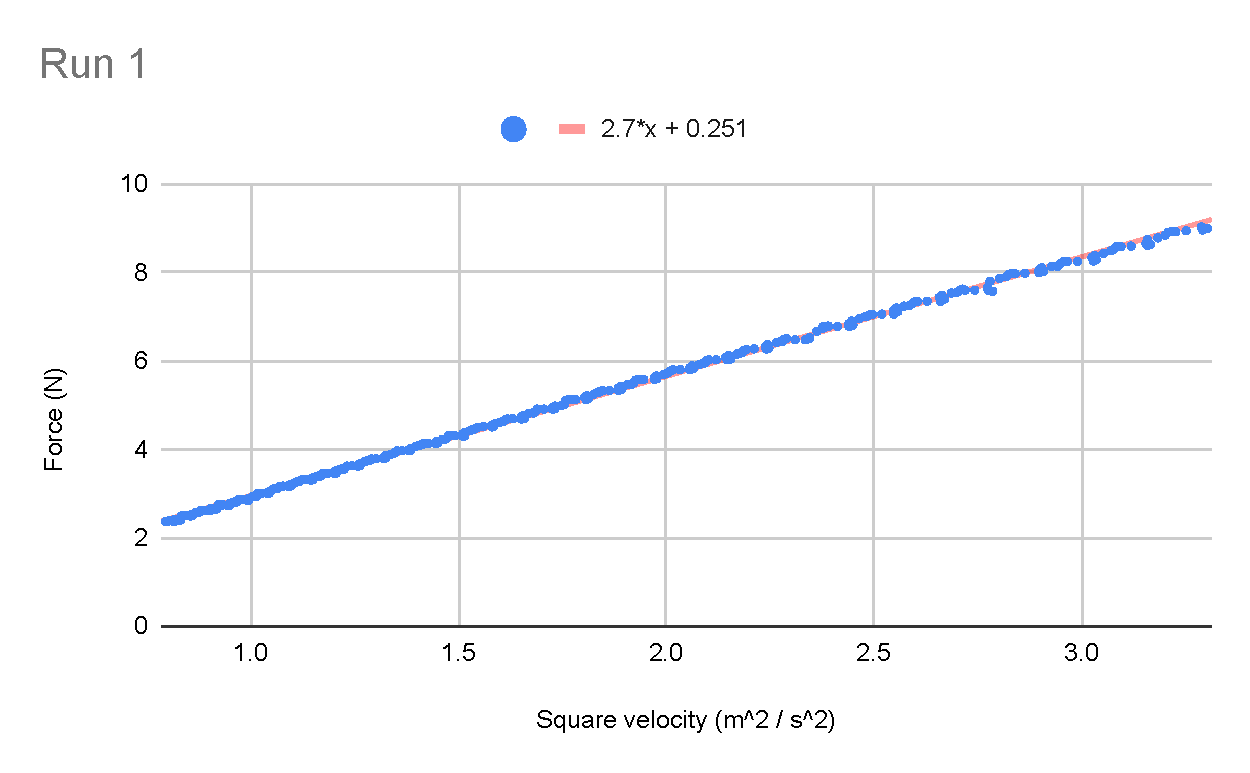
\includegraphics[scale=0.71]{image/10-centripetal/lab-6-Run-1.pdf}
    \end{center}
    \caption{Run 1}
    \label{fig:06.centripetal.run.1}
\end{figure}